\chapter{引言}

\section{RNA-Seq}
\nocite{wang2009rna, ozsolak2010rna}

RNA-Seq 是对 RNA 序列进行测量的一种技术, 
它是近几年来发展起来的通过深度测序用于研究转录组的一种技术. 
与其他的方法相比起来, RNA-Seq 揭露了生物的转录组中更多的复杂性. 
同时, RNA-Seq 能够更好地研究生物的转录组中各转录本的表达量. 
通过了解细胞中在某种特定条件下转录组中的转录本的组成, 
以及每一个转录本的表达量, 我们可以了解基因上的不同的功能模块, 
进而了解生物的发育过程, 以及疾病与人体之间的关系. 
通过使用 RNA-Seq, 我们已经对编码蛋白质的基因以及它们的剪切异构体 (isoform) 有了更为深入的了解. 
此外, RNA-Seq 也帮助我们对于基因上的非编码区域有了更为深入的认识, 
例如 lncRNA (long non-coding RNA).
并且我们对 sRNA (small RNA), microRNA 等也有了更全面的了解. 
\cite{pickrell2010understanding, encode, nagalakshmi2008transcriptional, 
tang2009mrna, banfai2012long, mortazavi2008mapping, wang2008alternative, 
katz2010analysis, deng2011isoform, lu2010function, mercer2011targeted, 
howald2012combining, lalonde2011rna, djebali2012landscape, 
derrien2012gencode, gerstein2012architecture, fairfax2012genetics, 
morrissy2011extensive, howald2012combining, park2012rna, 
tilgner2012deep, orom2010long, mercer2011human, chung2011computational, 
gingeras2009implications, roy2010identification, axtell2011vive, 
berezikov2010evolutionary, cherbas2011transcriptional, anders2012detecting, 
stoeckius2009large, lau2009abundant}

在 RNA-Seq 技术出现之前, 人们主要通过微阵列 (microarray) 对转录组进行定量分析和研究 \cite{schena1995quantitative}. 
但是与 RNA-Seq 相比, 微阵列存在若干问题 \cite{wang2009rna}: 
\begin{itemize}
\item 微阵列只能在序列已知的情况下使用

\item 结果会受交叉杂交 (cross-hybridization) 影响 \cite{okoniewski2006hybridization, royce2007toward}

\item 测量的表达量范围有限
\end{itemize}
另外, 在 RNA-Seq 技术出现之前, 人们主要通过 Sanger 测序法对互补 DNA (cDNA) 序列或者表达序列标签库 (EST libraries) 进行测序来研究转录组的序列 \cite{boguski1994gene, gerhard2004status}. 
但是 Sanger 测序价格昂贵, 同时测序通量偏低, 无法对转录组进行定量分析和研究. 
高通量测序技术的发展使得我们能够在较短的时间内用较少的成本对大量序列进行测序, 
几乎完整地测量转录组的序列, 
同时建立测序数量和实际被测序分子的数量间的关系 \cite{marioni2008rna}. 
这些是 RNA-Seq 在当今被广泛应用的一个主要原因. 

\begin{figure}[!t]
\centering
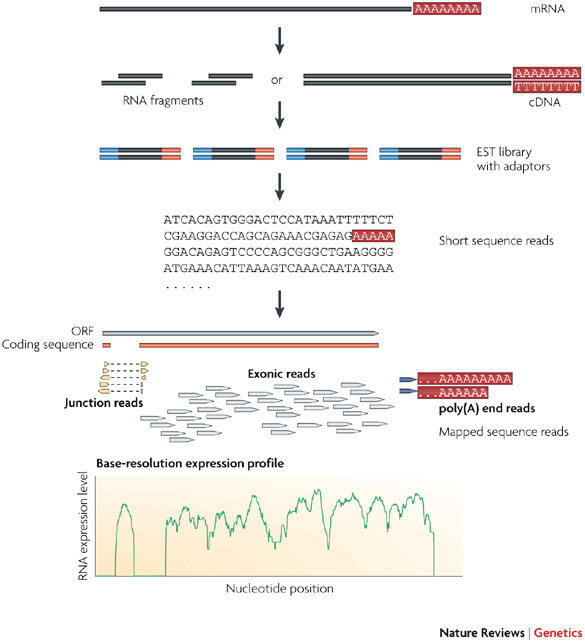
\includegraphics[width=\textwidth]{figures/rna-seq-experiment.jpg}
\caption{一般的 RNA-Seq 实验流程 \cite{wang2009rna}}
\label{intro-rna-seq-ex}
\end{figure}

\section{RNA-Seq 数据分析方法简介}
RNA-Seq 通常直接用于对于这些生物问题的研究:
\begin{itemize}
\item 发现新的剪切异构体 \cite{merkin2012evolutionary, wang2010novo, roberts2011identification, wang2010mapsplice}

\item 研究 RNA 序列的对于生物的调控作用 \cite{van2011xuts}

\item 比较不同条件下转录组不同的构成 \cite{trapnell2012differential}
\end{itemize}
同时, RNA-Seq 数据还未研究其他生物问题提供了宝贵的原始数据, 
例如对于生物系统中的网络的研究 \cite{sinicropi2012whole}. 

为了能够通过 RNA-Seq 数据对生物问题有深入的研究, 
我们通常会对 RNA-Seq 数据用这些方法进行处理:
\begin{itemize}
\item 序列比对 (sequence alignment): 将 RNA-Seq 读段找到其在基因组中的位置

\item 序列拼装: 
直接将 RNA-Seq 读段拼装成原转录组的各转录本. 若拼装时不依赖已知的参考序列, 
则成为 \textit{de novo} 拼装 ((\textit{de novo} assembly)). 

\item 各转录本的表达量估计: 用一定的单位表示每个被测样本中转录组里每个转录本的含量, 
用于在不同的样本之间进行比较

\item 辨识同一个基因的不同的剪切异构体: 真核生物中由于选择性剪切同一个基因会产生多个剪切异构体, 
通过 RNA-Seq 数据在一定条件下可以辨识出一个基因的不同的剪切异构体
\end{itemize}

\subsection{序列比对}
经典的序列比对算法包括 Smith-Waterman 算法 \cite{SmithWaterman1981} 和 Needleman-Wunsch 算法 \cite{needleman1970general}. 
但是由于 Smith-Waterman 算法和 Needleman-Wunsch 算法复杂度偏高, 它们不适用于大规模的数据. 
目前人们一般采用一些启发式的方法进行序列比对 \cite{isaev2004introduction}. 
对于将 RNA-Seq 读段比对到其在基因组中的位置, 目前比较常用的工具包括: 
\begin{itemize}
\item BLAT \cite{kent2002blat}
\item TopHat \cite{trapnell2009tophat}
\end{itemize}

\subsection{序列拼装}
序列拼装是生物信息学和计算生物学中一个经典的问题, 
其目的是通过测序的读段恢复出原始的生物序列. 对于序列拼装, 目前人们主要采用一下这两种常用的策略: 
\begin{itemize}
\item OLC (overlap-layout-consensus) \cite{greenphrap, bonfield1995new, 
kececioglu1995combinatorial, myers1995toward, huang1999cap3}

\item de Bruijn 图 \cite{pevzner2001eulerian}
\end{itemize}
目前对于 RNA-Seq 数据的拼装主要有这些常用的工具: 
\begin{itemize}
\item Cufflinks \cite{cufflinks.2010}: 
从 RNA-Seq 拼装转录组中的转录本时使用 OLC 策略 (图 \ref{intro-cufflinks-assembly})

\item Trinity \cite{grabherr2011full}: 
从 RNA-Seq 拼装转录组中的转录本时使用 de Bruijn 图策略 (图 \ref{intro-trinity-assembly})
\end{itemize}

\begin{figure}[!t]
\centering
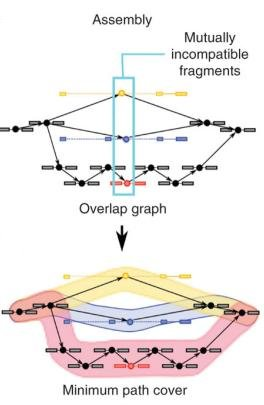
\includegraphics[height=0.5\textheight]{figures/cufflinks-assembly.jpg}
\caption{Cufflinks 序列拼装策略 \cite{cufflinks.2010}}
\label{intro-cufflinks-assembly}
\end{figure}

\begin{figure}[!t]
\centering
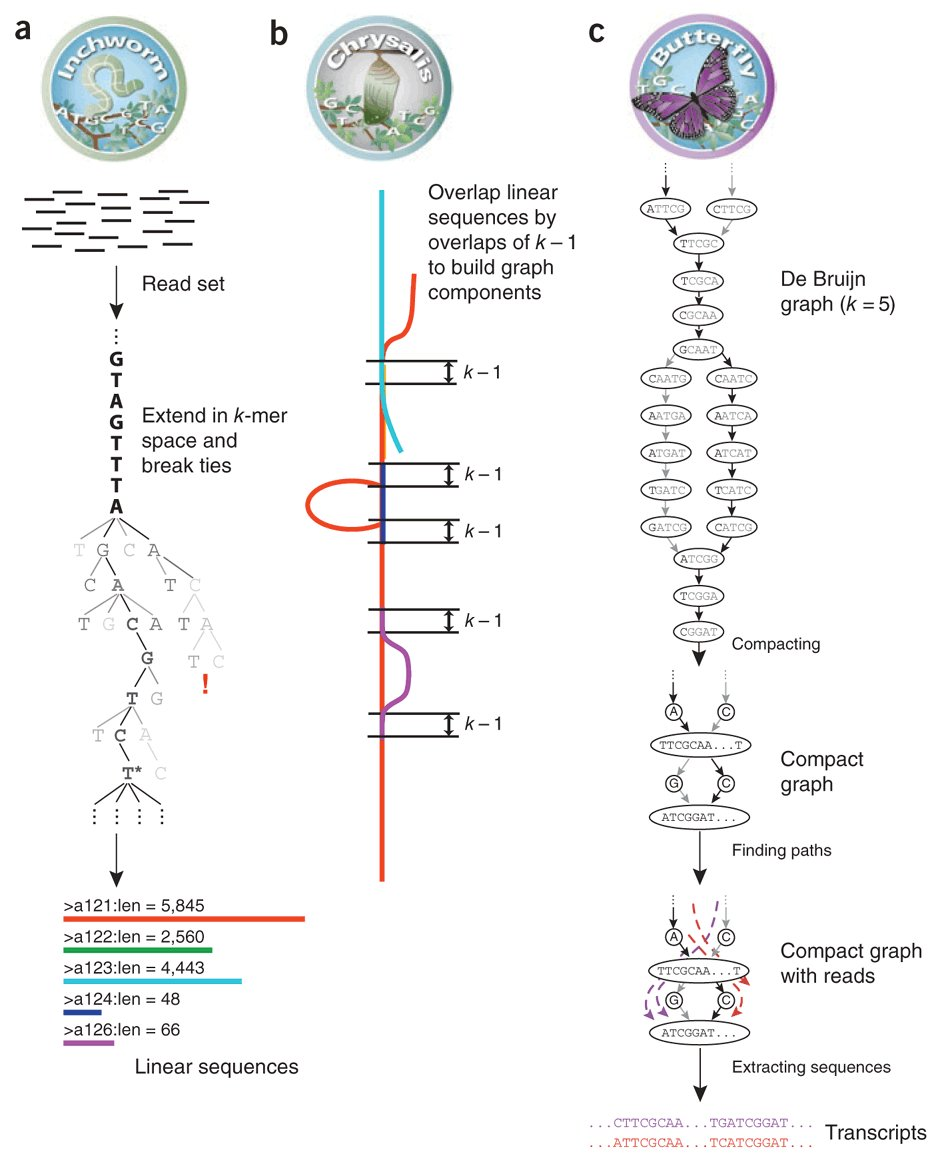
\includegraphics[width=\textwidth]{figures/trinity-assembly.jpg}
\caption{Trinity 拼装策略 \cite{grabherr2011full}}
\label{intro-trinity-assembly}
\end{figure}

\subsection{各转录本的表达量估计}

\subsection{辨识同一个基因的不同的剪切异构体}

\section{现有 RNA-Seq 数据定量分析方法}


